\begin{recipe}
    [% 
        preparationtime = {\unit[10]{min}},
        portion = {\portion{2}},
        bakingtime = {\unit[15]{min}}
    ]
    {Broccoli pesto}

    \introduction{%
        My grandma who cooks only traditional food fell in love in this pesto.
        I can recommend it more!
    }

    % \setRecipeLengths{
    %     ingredientswidth=10cm
    % }
    % TODO: Magda: ingredient names should be short.
    % Please move processing descriptions like chopping or pressing to the actual recipe.
    % This looks better and is easier to format.
    % The above command tweaks width of the ingredients pane.

    \ingredients[13]{%
        1 & Broccoli with stem \\
        \unit[0.75]{c.} & Olive oil \\
        \unit[1]{c.} & Roasted almond (or sunflower seeds) \\
        4-5 & Garlic cloves \\
        1 & Onion, diced \\
        2cm & Ginger, diced \\
        3 & Garlic cloves, diced/pressed \\
        \nicefrac{1}{2} bunch & Parsley \\
        \unit[5]{ts.} & \underline{Yeast flakes} \\
        & Chili \\
        & Nutmeg \\
        & Lemon juice \\
        & salt\&pepper
    }

    \preparation{%
        \step Cut broccoli into pieces, cook on boiling water for 4-5 min.
        Drain and cool with cold water (preserve nice green colour).
        \step Blend everything.
        \step Voilà!
    }

    \suggestion{%
        Serve with pasta, topped with cheese and cherry tomatoes.
        Or serve with bread.
        Or even with roast (as sauce) or raw vegetables (as dip).
    }

    \hint{%
        To roast almonds (or any other seeds/nuts), preheat the frying pan well (the thicker the frying pan, the better (eg cast-iron)), do not add any fat.
        Keep it at high heat, stir from time to time (not too often, though!
        Let them roast).
        Remember to transfer them immediately to a bowl/suitable tupperware as the frying pan is still hot after turning the hob off.
    }

\end{recipe}

\begin{figure}[t]
    \centering
    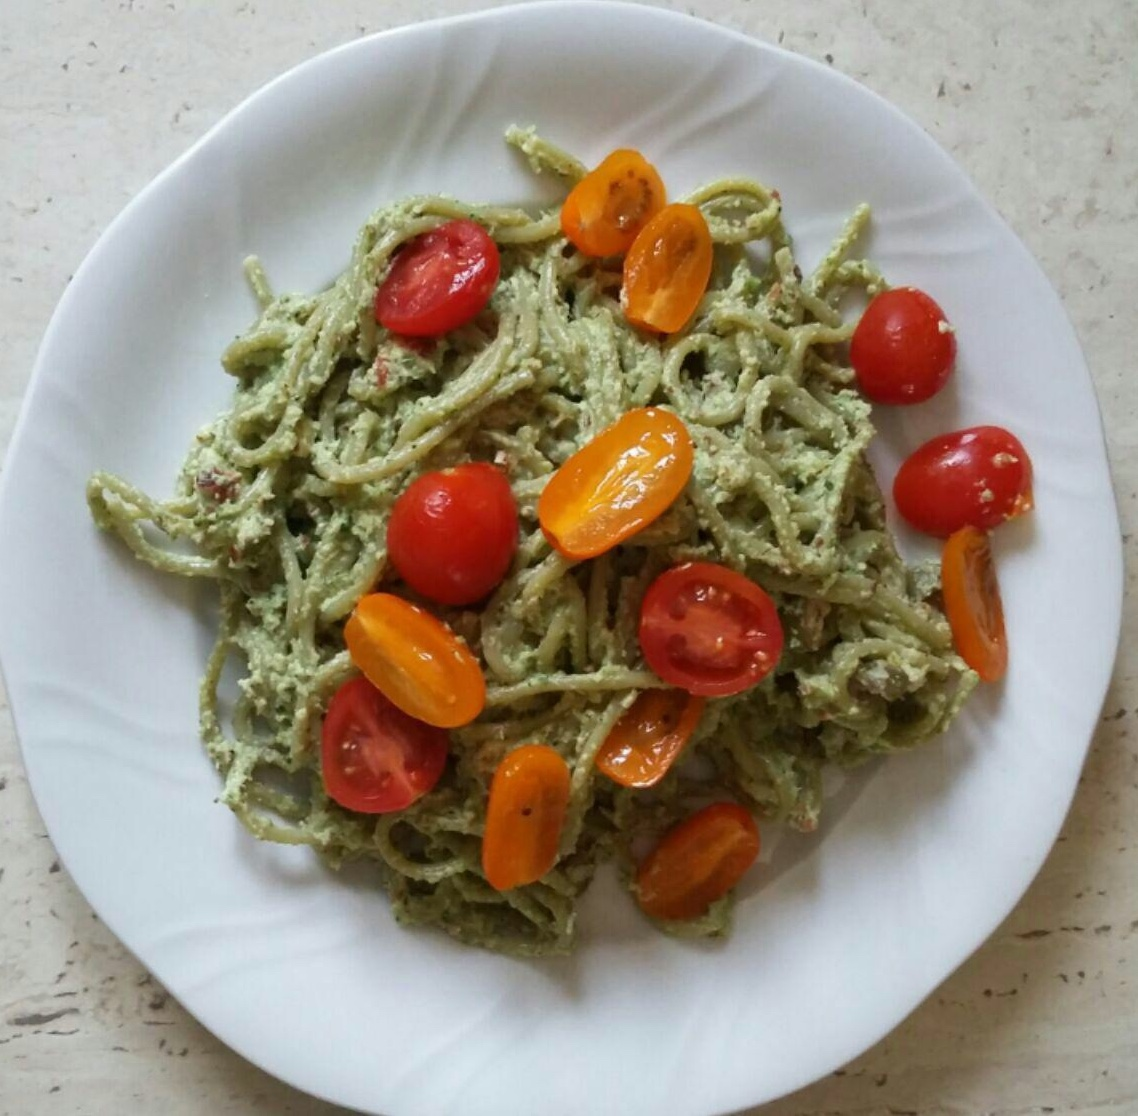
\includegraphics[width=12cm]{pic/brocolli_pesto}
\end{figure}
